\documentclass[prl,aps,twocolumn,floatfix,amsmath,amssymb,superscriptaddress,tightenlines]{revtex4}
\usepackage{graphicx}
\usepackage{epstopdf}
\usepackage{amsfonts}
\usepackage{bm}
\usepackage{color}
\usepackage{ulem}
\begin{document}

\newcommand{\be}{\begin{equation}}
\newcommand{\ee}{\end{equation}}

\date{\today}
\title{Universal large-scale entanglement in
  two-dimensional gapless systems}

\author{Hyejin Ju}
\affiliation{Department of Physics, University of California, Santa Barbara, CA, 93106}

\author{Ann B. Kallin}
\affiliation{Department of Physics and Astronomy, University of Waterloo, Ontario, N2L 3G1, Canada} 

\author{Paul Fendley}
\affiliation{Physics Department, University of Virginia,
  Charlottesville, VA 22904}
\affiliation{Microsoft Research, Station Q, CNSI Building, University of California, Santa Barbara, CA, 93106}

\author{Matthew B. Hastings}
\affiliation{Microsoft Research, Station Q, CNSI Building, University of California, Santa Barbara, CA, 93106}

\author{Roger G. Melko}
\affiliation{Department of Physics and Astronomy, University of Waterloo, Ontario, N2L 3G1, Canada} 

\begin{abstract} 
We numerically determine universal terms in the entanglement entropy of several two dimensional (2D) gapless systems, including a Heisenberg model with N\'eel order, a free Dirac fermion, and the nearest-neighbor resonating-valence bond wave function.
For these models, we show that the entanglement entropy between regions of length $x$ and $L-x$ extending around a torus of
length $L$ depends upon the dimensionless ratio $x/L$, and can be well-approximated on finite-size lattices by a function
$\ln(\sin(\pi x/L))$, akin to the ``chord-length'' in one dimension.
\sout{We consider the role of the toroidal aspect ratio and we find that an additive logarithmic divergence in $L/a$, where $a$ is the lattice scale, appears in some models but not others.}  The presence of an additive logarithmic divergence in the Dirac fermion for different toroidal aspect ratios hints however that the precise form of this function may differ from the chord-length in the thermodynamic limit in 2D.
\end{abstract}
\maketitle

{\it Introduction.} Quantum condensed matter systems, long studied with a host of probes related to energy spectrum, broken symmetry,
and fluctuations, are now benefitting from a infusion of ideas related to quantum information and entanglement.
%order parameters, correlation functions and similar, are now clearly This paradigm is highlighted best with the study of entanglement entropy scaling.  
The importance of this new resource is most strikingly 
demonstrated in the study of entanglement entropy at conformally-invariant 1D quantum critical points.
%It is now well established that the low-energy
%physics of many one-dimensional (1D) quantum many-body systems can be
%described by relativistic 1+1 dimensional field theories.  This
%correspondence is common at quantum critical points, 
%where in addition
%to scale invariance, quantum systems may enjoy {\it conformal}
%invariance. 
Here, their relation to conformal field theory (CFT) provides an important
universal number, the {\it central charge} $c$, that appears in an astonishing array of physical
quantities \cite{Cardyubiquitous}. A given CFT, and
thus any quantum critical points it describes, can be
characterized by this number,
%Moreover, a profound result, Zamolodchikov's
%$c$-theorem, indicates that $c$ cannot increase in
%renormalization-group flows \cite{Zamo}. 
which thus provides a valuable tool in identifying which if any conformal field
theory describes a given Hamiltonian. 
%Namely, since it appears in
%various physical quantities, it can be measured numerically, and then
%compared with the central charges of the (many) known
%CFTs. 
\textcolor{red}{Traditionally, extracting $c$ numerically for a 1D quantum
Hamiltonian was done by analyzing the finite-size spectrum
\cite{BCN,Affleck}.  This can be difficult: not only is it a
subleading contribution to the ground-state energy, but it requires also
determining the Fermi velocity.}
%More recently, a more direct method very amenable to numerical
%simulation has been utilized.  
However, it was demonstrated \cite{Holzhey, VidalC} that the central charge can also be extracted 
directly from the ground-state wavefunction by measuring its Renyi
entanglement entropy, $ S_n = 1/(1-n) \ln \big[ {\rm Tr} \rho_A^n
\big], $ where region $A$ is entangled with its complement, region
$B$.  In particular, the scaling of the Renyi entropy at a 1D critical system,
with total length $L$ and length of region $A$ being $x$, obeys a ``chord-length''  \cite{Korepin,Cardy},
\begin{equation}
S_n = \frac{c}{6}\left({1+ \frac{1}{n} }\right) \ln\Big[ \frac{L}{\pi} \sin\big( \frac{\pi x}{L} \big) \Big]. \label{1Dcft}
\end{equation}
\sout{Here, $c$ appears as the coefficient of the leading term.  }
Numerical measurements of entanglement entropy have become commonplace and 
very accurate, e.g. in simulations using the density matrix renormalization group,
making Eq.~(\ref{1Dcft}) the gold standard for identifying $c$.


In higher dimensional ground states of condensed matter systems, the scaling behavior of
entanglement entropy is much less well-understood.  Local Hamiltonians
are generally believed to produce an ``area-law'' (i.e. boundary) scaling, the subleading corrections
to which may be universal quantities that can be used to identify and characterize
quantum phases and phase transitons.
The most well established of these is the {\it topological entanglement entropy} \cite{KP,LW} of a gapped
spin liquid state, that is, a universal quantity reflecting the emergent gauge symmetry.
In gapless states, the subleading corrections, although still potentially harboring universal 
quantities, become more complicated \cite{Misguich}.
In presence of spontaneously broken continuous symmetry, it has been found that Goldstone modes 
produce a bulk logarithmic correction \cite{HeisLog,MaxLog}.
Subleading logarithms are also predicted to occur at critical points, the coefficients of which are universal \cite{logcorner,Max}.
%In higher dimensions, the relationship between entanglement entropy
%and universal quantities is less concrete.  Although conformal
%invariance exists at scale-invariant critical points in the presence
%of translational and rotational symmetry, the breaking of these
%symmetries in physical systems can make the critical points
%non-conformal.  Moreover, even if conformal, precisely which quantity
%in general to identify as a central charge is an open question.
Some speculate that the presence of logarithmic scaling can be used to define an ``effective'' central
charge for non-conformally invariant systems in 2D. % that may contain
%universal physics (or perhaps even the equivalent of the $c$-theorem
%in higher-dimensions \cite{ryu,Myers}).  
%Arguments exist that logarithms similar to Eq.~(\ref{1Dcft}) should emerge due to some
%asymptotic restoration of conformal invariance in higher-dimensional
%gapless models \cite{Shredder} (although counter examples are known).  
However, as Calabrese and Cardy caution, basic scaling relationships of
higher-dimensional systems need to be carefully checked before
arguments about asymptotic restoration of conformal invariance are
advanced \cite{EE_CFT}.

In this paper, we study numerically the scaling of the second Renyi entropy in several gapless wavefunctions in 2D.
For a free spinless fermion in the $\pi$-flux phase, we find that the entanglement scaling has a universal shape-dependent piece.
For finite-size systems, this closely mimics the chord length of Eq.~(\ref{1Dcft}), although in the infinite-size limit 
it is observed to cross over to a different non-trivial function.
We also examine finite-size scaling of the Renyi entropy in the gapless N\'eel state, and the nearest-neighbor RVB wavefunction
on the 2D square lattice, using quantum Monte Carlo (QMC) simulations.
In addition to the subleading logarithm identified in Refs.~\cite{HeisLog,MaxLog},
we observe the emergence of a shape-dependent scaling function that closely mimics the chord-length of 1D CFT on finite-size systems, similar to the case of $\pi$-flux fermions.
Among other consequences, this shape-dependent term will give a non-zero signature in the entanglement quantities \cite{KP,LW} designed to look for topological order, which implies that a straightforward generalization a topological entanglement entropy will not be possible in gapless spin liquid states.



 \begin{figure}
   \begin{center}
   \scalebox{1}{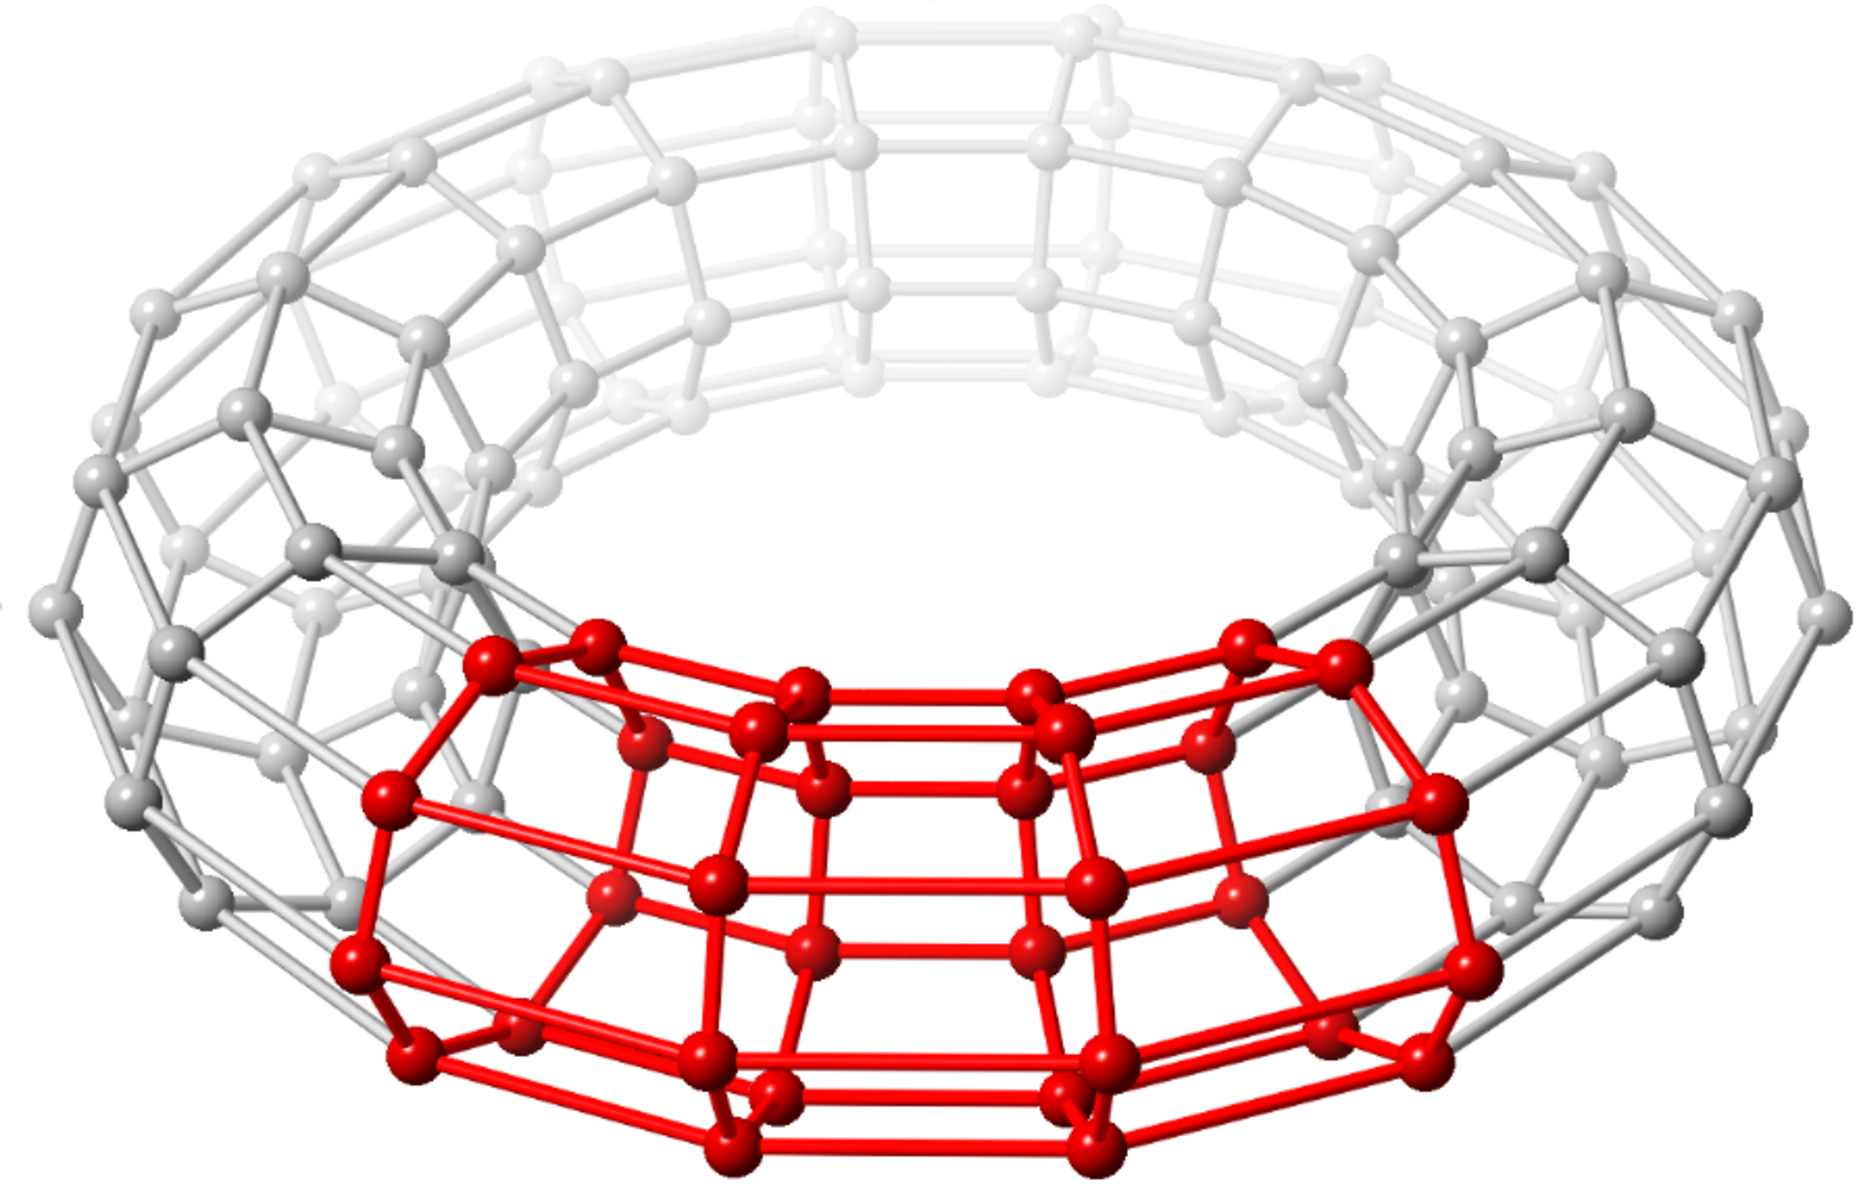
\includegraphics[width=2.1in]{./figs/16x8b.pdf}}
   \end{center}
   \caption{An $8 \times 16$ toroidal lattice.  The width of region $A$ (blue) is $x=4$.  The boundary length between region $A$ and its complement is $\ell = 16$. }
   \label{fig:torus}
 \end{figure}
 
%Since the terms in the Renyi entropy with
%universal behavior are subleading in $d>1$, it has only recently become
%possible to measure them accurately through the development of measurement
%techniques in scalable quantum Monte
%Carlo (QMC) methods \cite{swap,XXZ}.  Simulations employing this advance
%have confirmed the presence of universal subleading corrections to the
%area-law in topologically-ordered systems \cite{isakov}, as well as preliminary
%confirmations of area-law (and subleading logarithms) in the simple
%gapless 2D N\'eel state \cite{HeisLog}. %>>> Misguich should be mentioned too, they've been doing this for a while???.  
%In this paper, we perform a careful
%finite-size scaling analysis of Renyi entropies in a specific
%cornerless geometry in several gapless wavefunctions \cite{Misguich}. 

{\it Fermions with $\pi$-flux---}
%Before presenting the quantum Monte Carlo (QMC) analysis of more complicated models, we begin with a more tractable case, a free fermion model.
We begin by considering a tractable case of
free spinless fermions on a square lattice, with $\pi$-flux through each plaquette.  We consider a torus of size $L_x$ by $L_y$, and
measure the entanglement % for two different types of region $A$: a $square$ region $A$ containing four corners, and 
using a cornerless $strip$ region $A$ (Fig.~\ref{fig:torus}) which has no corners and constant boundary length $\ell = 2L_y$.
We denote the width of region $A$ by $x$ and $L = \ell/2$.
%, where a square will have dimensions $x$ by $x$ and a strip will be $x$ by $L$ when it is embedded in an $L$ by $L$ system.
Using translation invariance in the $y$-direction, it is possible to simulate large systems.  This system has Dirac points near momentum $k_y=0$ and $k_y=\pi$.  We take anti-periodic boundary conditions in the $x$-direction so that there will be no exact zero mode.

We claim that the entanglement entropy of such a system is given by
\be
S_n \sim {\rm const.}\times \ell + F(x/L_x,L_y/L_x),
\ee
where the constant is non-universal and the function $F$ is a universal scaling function of the dimensionless ratios.  Note that this result differs
from the result in one dimension, Eq.~(\ref{1Dcft}), in that the lattice scale appears in the first non-universal term but does not appear in the second universal log.  In contrast, the one-dimensional result can be written as a sum of two terms as:
$S_n = \frac{c}{6}\left({ \frac{1}{1+n} }\right) \ln[\sin\big( \frac{\pi x}{L} \big)]+\frac{c}{6}\left(\frac{1}{1+n}\right)\ln[\frac{L}{\pi}]$, so that the first term is a universal function of the dimensionless ratio $x/L$, akin to the function $F$ above while the second term involves the lattice scale, as it diverges with $L$.

To illustrate the absence of such an ``additive logarithm" (a logarithmic divergence depending on $L$ divided by lattice scale) in two dimensions, it is helpful to 
consider the two-dimensional entropy as a sum of one-dimensional entropies of systems with different momenta, $k_y$.  Let $C=(c/6)(1+n)^{-1}$.  Then, the $k_y=0$ mode has an additive logarithm $C \log(L_x)$.  The modes with small $k_y \neq 0$ have additive logarithms $C \log(k_y^{-1})$ (a more precise calculation would include the effect of a finite $L_x$ for these modes; we ignore this here as our only goal is to show the cancellation of additive logarithms).  Summing over $k_y=2\pi n/L_y$, this gives an entropy (in this crude approximation) $C \big( \log(L_x)+\sum_{n=1}^{L} \log(L_y/2 \pi n) \big)=C\log(L_x) + C\log((L_y/2\pi)^L_y/L_y!)$.  Using Stirlings formula for $L_y!$, one finds that the additive logarithm terms add to $C(\log(L_x)-\log(L_y))=C\log(L_x/L_y)$ which can be absorbed into the scaling function $F$, so that there is no additive logarithm.  A similar calculation near $k_y=\pi$ leads to a cancellation of the additive logarithm there.
\textcolor{blue}{In contrast to this case, we will find below that such an additive logarithm {\it is} present for the Heisenberg system \cite{HeisLog}.}

The entropy of a given $k_y$ mode contains, in addition to the additive logarithmic divergence in $k_y$, a universal scaling function $G(x/L_x,k_y x)$.  At $k_y=0$, we see the chord-length scaling $C \ln\sin\big( \frac{\pi x}{L} \big)$ (Fig.~\ref{fig:dirac}), but for $k_y \neq 0$ and for $k_y x$ large, the chord-length scaling disappears and the entropy becomes roughly flat as a function of $x/L$.  In fact, for $L_y=L_x=L$, the lowest $k_y$ mode has a mass $2 k_y=4\pi/L$, and hence the entropy of that mode is flat for a large range of $x/L$.  As a result, for $L_y=L_x=L$, the entropy of the two dimensional system appears to display 1D chord length scaling over a wide range of $x/L_x$.

 \begin{figure}
   \begin{center}
   \scalebox{1.7}{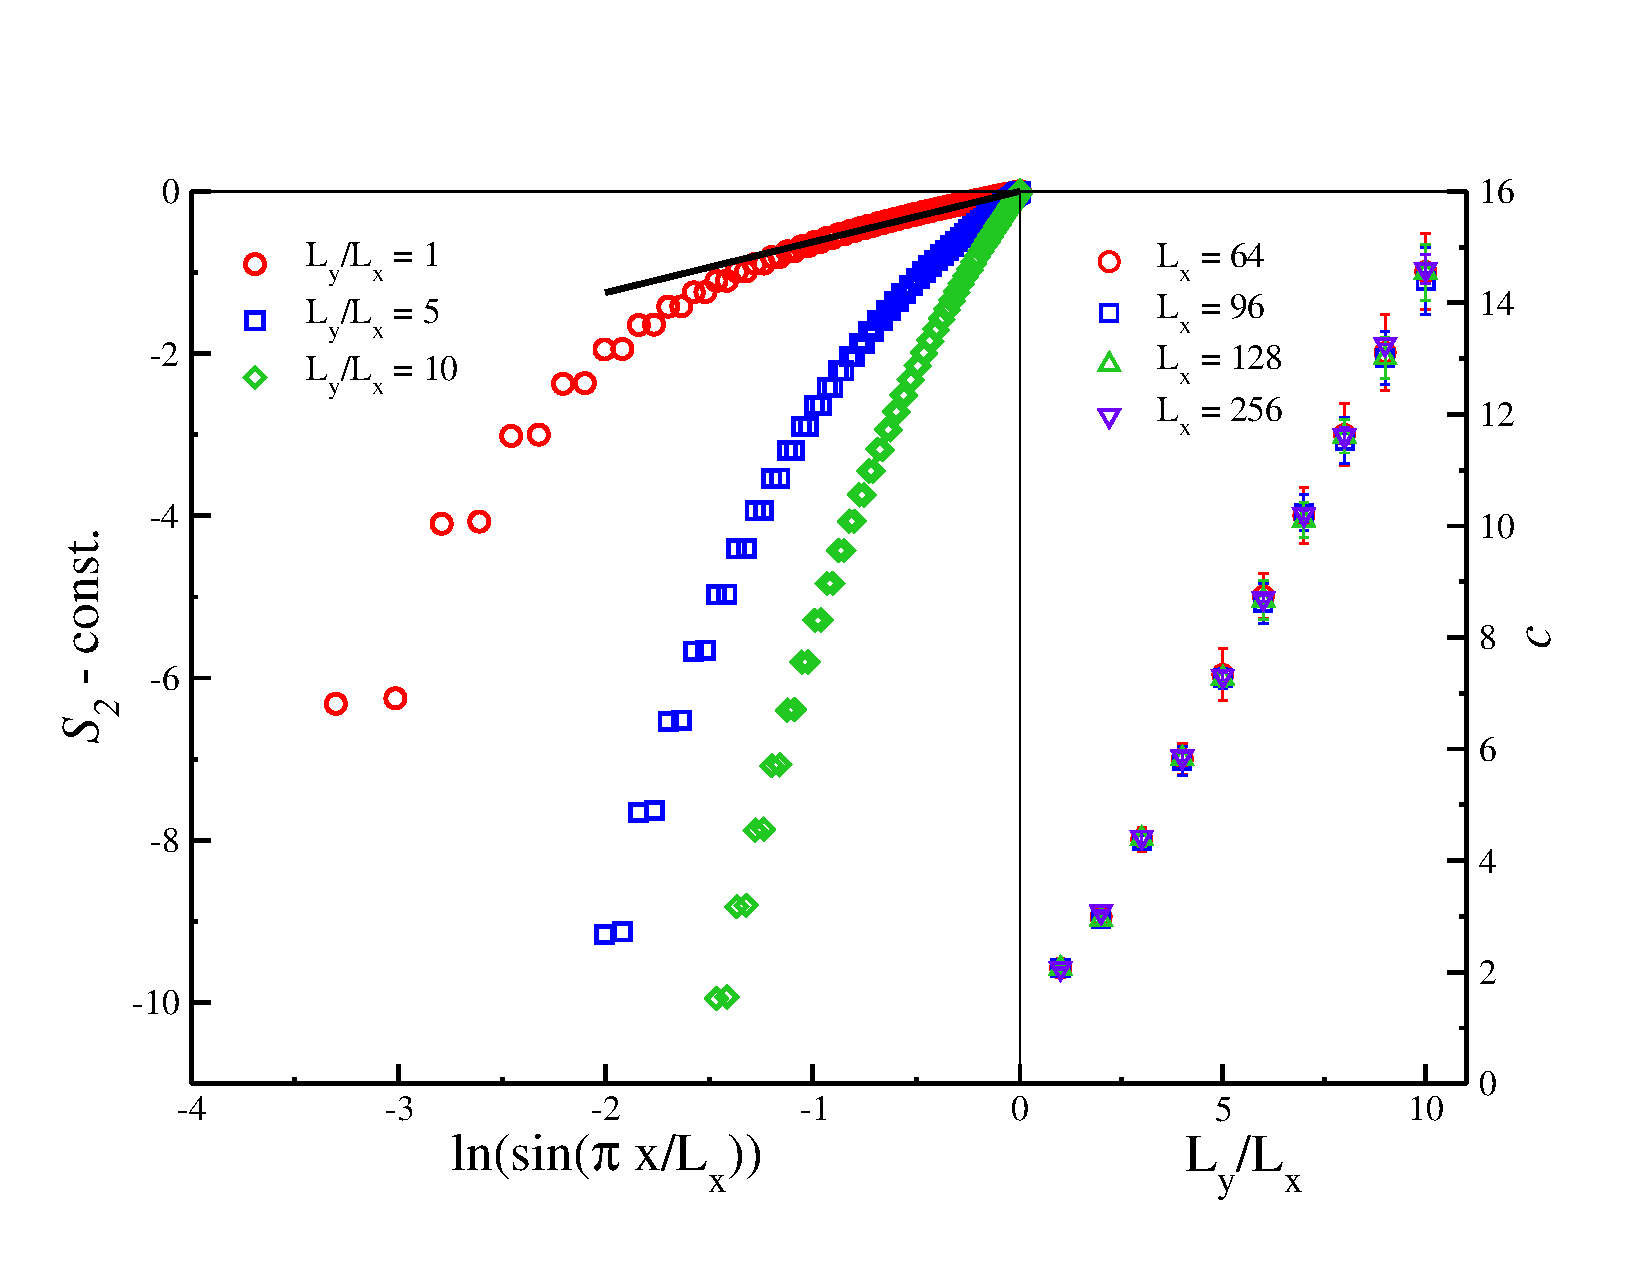
\includegraphics[width=2.1in]{./figs/dirac/fermion.pdf}}
   \end{center}
   \caption{Entanglement entropy of $L=256$ Dirac fermion model. The curve is less linear at larger $L_y/L_x$.}
   \label{fig:dirac}
 \end{figure}
 
{\it Quantum Monte Carlo---}
Using QMC techniques we simulate both the
Heisenberg ground state and the resonating valence bond (RVB)
wavefunction in two dimensions (2D).  The Heisenberg ground state is
projected from a trial state by applying a high power of the
Hamiltonian, $H = \sum_{\langle ij \rangle} {\bf S}_i \cdot {\bf S}_j$, via a QMC method operating in the valence bond (VB)
basis \cite{Sandvik}. %The Hamiltonian operators act to reorganize the
%bonds while effectively penalizing states with longer bonds.  
The RVB wavefunction, in contrast, 
is composed of a linear superposition of all possible 
nearest-neighbor valence-bonds \cite{RVB1,RVB2},
\begin{equation}
| \Psi \rangle = \sum_{\alpha} | V_{\alpha} \rangle,
\end{equation}
where
\begin{equation}
|V_{\alpha} \rangle =  \frac{1}{2^{N/4}} \prod_{i=1}^{N/2} \big( | \uparrow_i \downarrow_{j_{\alpha}} \rangle -  | \downarrow_i  \uparrow_{j_{\alpha}} \rangle \big)
\end{equation}
contains the spin basis associated with a valence-bond singlet $\alpha$.
The RVB 
Monte Carlo sampling
algorithm does a random walk through the possible states by creating a
defect at some spatial point and propagating it through the system (thereby
rearranging the nearest-neighbor bonds) until the defect reaches the
initial point and its path forms a closed loop \cite{AWSloop}.
If we visualize the Heisenberg ground state in this VB language, then the RVB wavefunction is its largest component, the remainder of the state being equal superpositions with longer bonds decaying with the length of the bonds as $1/r^3$ \cite{Sandvik}.
We consider the same geometry as for the $\pi$-flux fermions above, with $L_x=L_y=L$ (see Fig.~\ref{fig:torus}).

 \begin{figure}
   \begin{center}
   \scalebox{1}{\includegraphics[width=0.9\columnwidth]{./figs/rvb-heisenberg.pdf}}
   \end{center}
   \caption{ The second Renyi entropy for the N\'eel and RVB states for $L=24$. Notice that the entanglement entropy for the RVB splits into two branches, even and odd, which may be related to the existence of topological sectors of the underlying transition graphs.
   %Heisenberg strip data for $L=12,16,\dots,40$ with fits to the function $m\log(\tfrac{L}{\pi}\sin(\tfrac{x\pi}{L}))+h$} for each system size.
   \label{fig:heis_bow} }
 \end{figure}

In Fig.~{\ref{fig:heis_bow}} we illustrate QMC results for the Renyi entropy in the N\'eel and RVB states on a $24 \times 24$ torus.  
Several features of the entanglement scaling are clear from this plot.  First, note that the data for the N\'eel state has a significant curvature as a function of $x$.  This curvature, first seen in Ref.~\cite{HeisLog}, was not explored in detail in that work.  Rather, it was demonstrated that, by examining the finite-size scaling at $x=L/2$ as a function of $L$, a subleading logarithmic term $\propto \ln(\ell)$ is present, surprisingly, even with an absence of corners in the region $A$ \cite{MaxLog}.
%N\'eel state, first explored in Ref.~\cite{HeisLog}.  In that work, the presence of an area law term $\propto \ell$ was confirmed, as well as a subleading logarithmic term $\propto \ln(\ell)$ (present, surprisingly, even with an absence of corners in the region $A$).  This subleading term was extracted when the width of the region $A$, $x = L/2$, is equivalent to the ``center'' of each curve in Fig.~{\ref{fig:heis_bow}}.  
As is apparent, the choice $x=L/2$ removes the $x$-dependence of each curve in Eq.~(\ref{1Dcft}).  
Similarly, there is significant curvature in the $x$ dependence of the RVB wavefunction.  However, there exists a more complicated structure to the entropies than in the N\'eel state: the appearance of two branches, an ``upper branch'' when $x$ is odd, and a ``lower branch'' when $x$ is even.  We discuss this branching structure more below.

To capture the $x$-dependent curvature of these wavefunctions, we attempt to fit the data with the scaling ansatz
\begin{align}
S_2= a \ell + b\ln(\ell)
+ c(L) \ln \left[{ \sin\left({ \frac{\pi x}{L} }\right) }\right] + d \label{Fit}
\end{align}
motivated by the chord-length of Eq.~(\ref{1Dcft}).
We begin by examining the N\'eel state in Fig.~{\ref{fig:heis_lines}}.  For a fixed linear system size $L$, plots of $S_2$ versus $ \ln \left[{ \sin\left({ \frac{\pi x}{L} }\right) }\right] $ would yield a straight line if Eq.~(\ref{Fit}) were obeyed perfectly.  
One could speculate therefore that the apparent chord-length scaling of these square-lattice 2D systems is actually not perfectly obeyed in the thermodynamic limit, and that this fact is manifest in slight deviations from straight-line behavior in Fig.~{\ref{fig:heis_lines}}(a).
This would be a similar scenario to the deviation from chord-length scaling observed for $\pi$-flux fermions in Fig.~\ref{fig:dirac}.  
However, it is difficult to draw a firm conclusion regarding the statistical significance of any deviation from Eq.~(\ref{Fit}) scaling in our
present data, due to limited system sizes and stochastic error.

 \begin{figure}
   \begin{center}
   \scalebox{1}{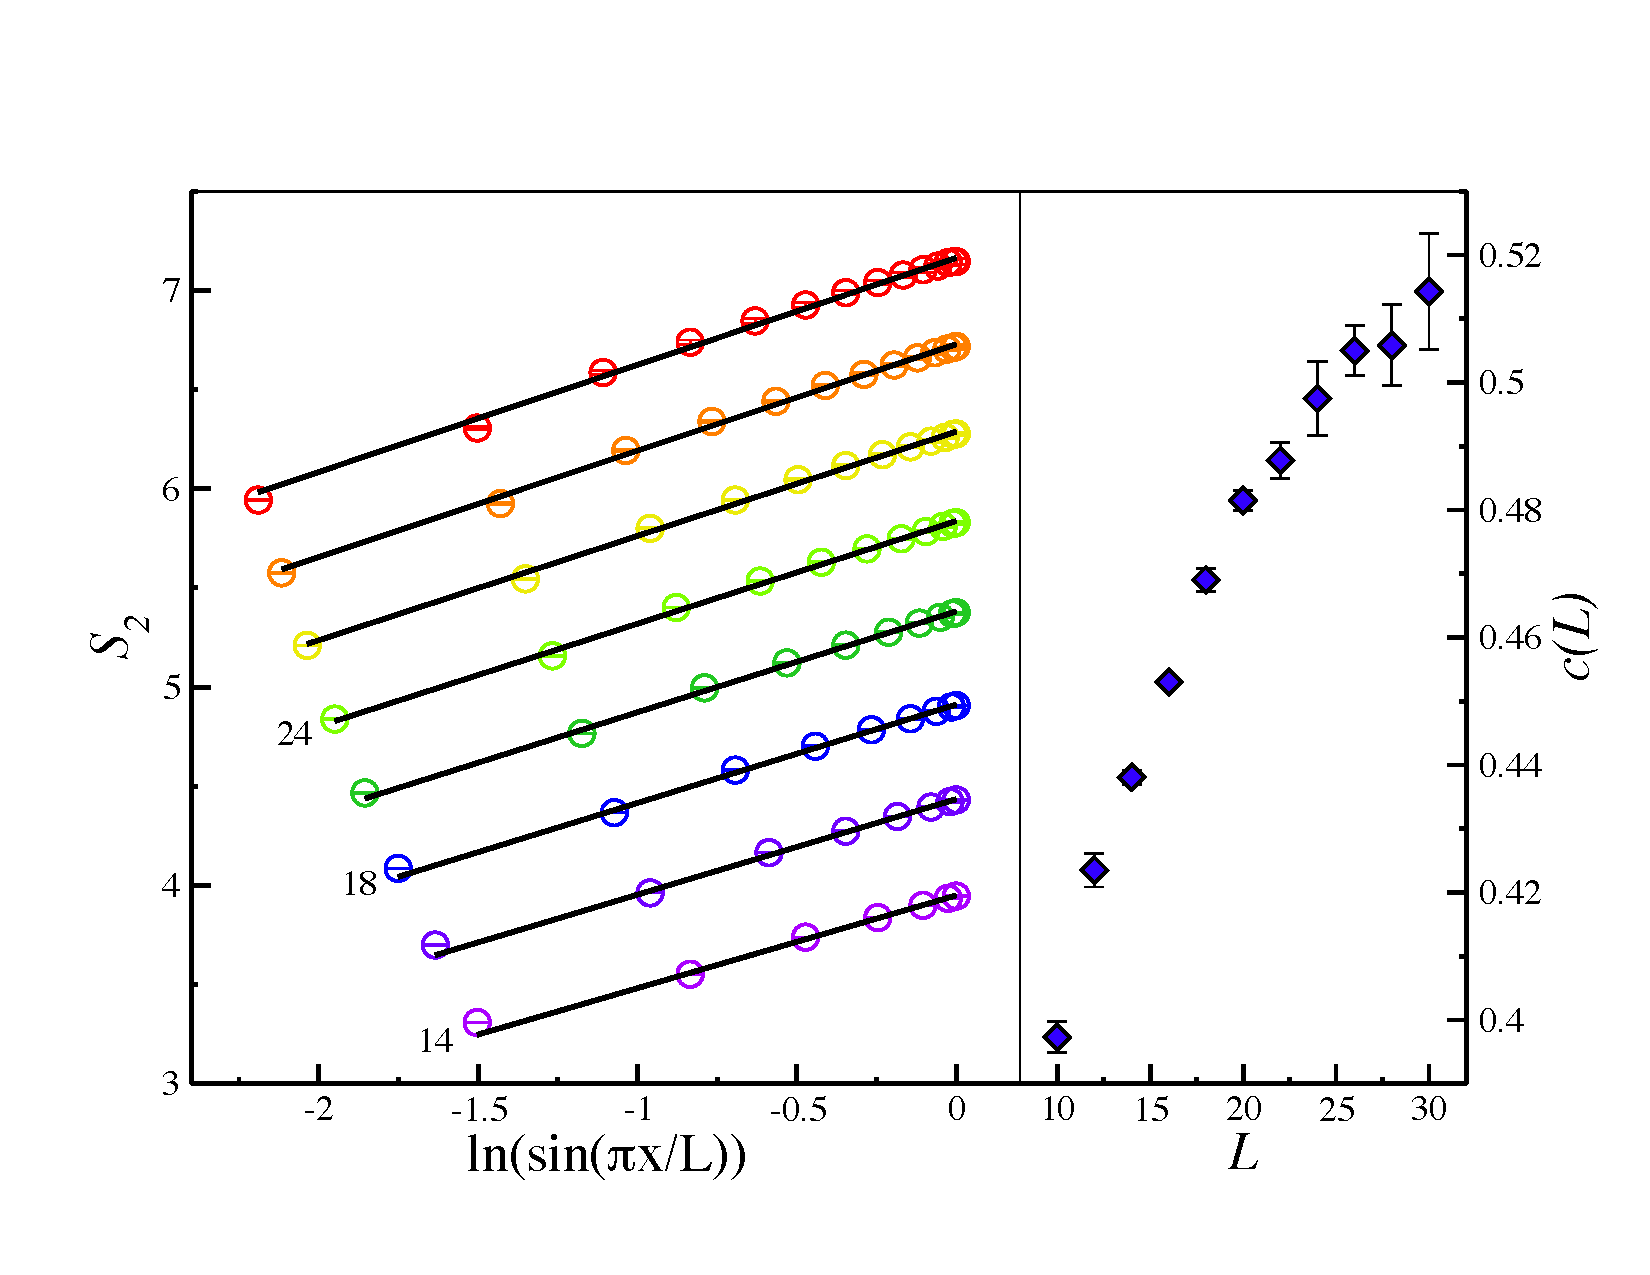
\includegraphics[width=\columnwidth]{./figs/heis.pdf}}
   \end{center}
   \caption{(a)Heisenberg data and linear fits (excluding the first two data points on the left) for $L=14,16,\dots,30$ plotted in terms of the log of the ``conformal distance", $\ln\left[\sin \frac{\pi x}{L}\right]$.
   (b) Slopes, $c(L)$, for each $L$ on the left.
   }
   \label{fig:heis_lines}
 \end{figure}

%In fact, as is visible in the largest $L$ considered, there is a slight deviation of the straight-line fits for small $x$.  
We can however further examine the deviation from conformal scaling by examining the universality of the 
coefficient of the chord-length in the N\'eel state.
To do this, we extract the $L$-dependence of the coefficient $c(L)$ in Eq.~(\ref{Fit}).  As illustrated in Fig.~\ref{fig:heis_lines}(b),
the coefficient does not approach a constant for the system sizes that we have studied, rather is has some functional dependence on $L$.
This functional dependence is apparently sub-linear.  It is interesting to speculate that $c(L) \sim L^p$ with $p<1$,
which could be accounted for \textcolor{blue}{by a mode-summing argument as in the gapless fermion case above that, in N\'eel case, 
resulting in an un-cancelled series of logs}.  A rigorous analysis of the data along this lines is impossible however within the current
accuracy of our QMC simulations.

%It is clear in that this form gives an excellent fit to the data for all $x$ and $L$, providing strong evidence for the presence of the chord length.  We can analyze the fits further by examining the dependence of the coefficients on system size $L$.  Most interestingly, we observe the coefficient of the chord-length increasing with $L$, as illustrated in the inset of Fig.~{\ref{fig:1}}.

 \begin{figure}
   \begin{center}
   \scalebox{1}{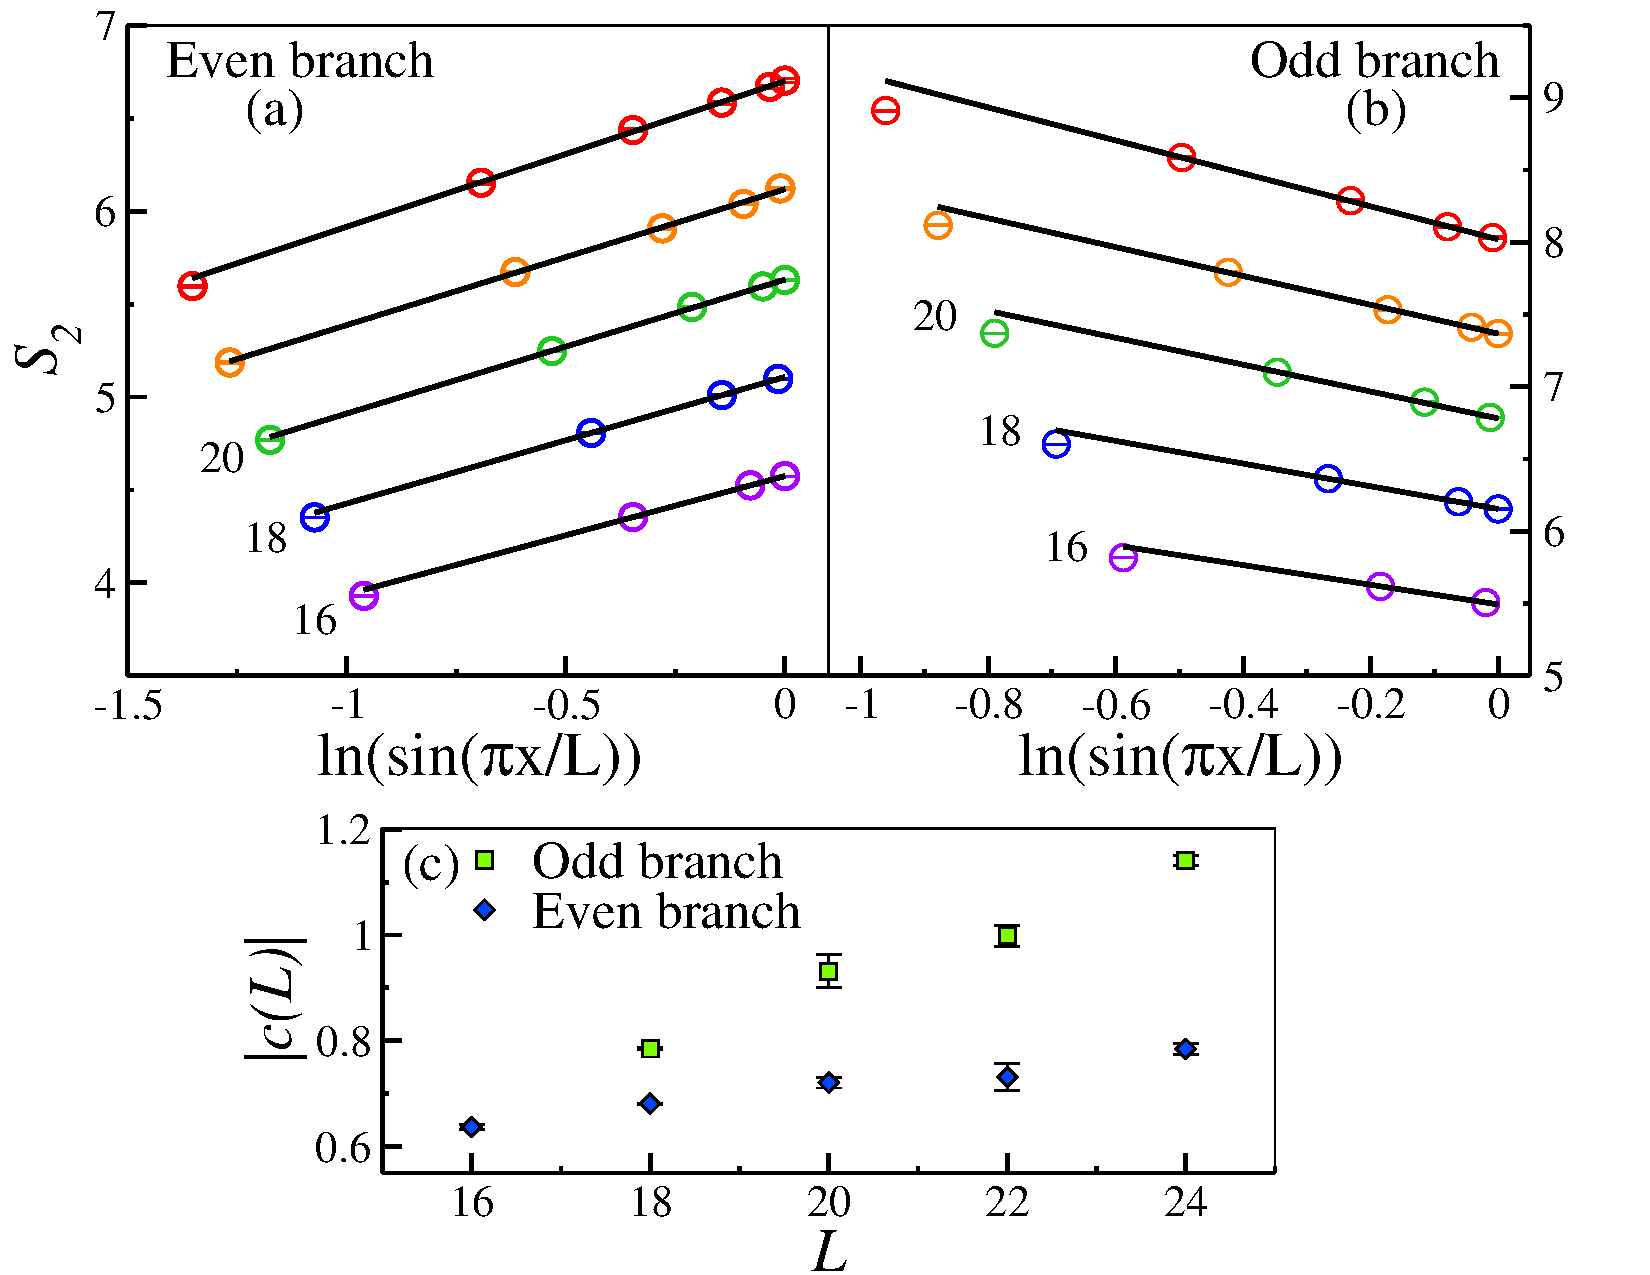
\includegraphics[width=\columnwidth]{./figs/rvb/rvb-bow.pdf}}
   \end{center}
   \caption{Preliminary RVB fig - (top left) Slopes from data in bottom panels, (top right) RVB $S_2$ for $L=24$ (excluding $x=1$ and $x=23$). (Bottom) RVB data for $L=12,16,20,24,28$ for even (left) and odd (right) values of $x$.}
   \label{fig:2}
 \end{figure}

We next examine the scaling of the Renyi entropy in the RVB wavefunction, illustrated in Fig.~{\ref{fig:2}}.  
As discussed above in Fig.~\ref{fig:heis_bow}, a very striking two-branch structure exists, depending on whether the distance $x$ is even or odd.
The precise source of the two branches is not known, although simple counting arguments of prototypical valence-bond configurations in the (0,0) topological \cite{RVB1,RVB2} sector may hint at their existence, since the number of valence-bonds crossing from region $A$ to region $B$ alternates strongly with $x$.  Even from this $L=24$ data there is a clear $x$-dependent curvature in each branch: this can be analyzed more closely by examining one branch and attempting fits of the form Eq.~(\ref{Fit}).  

In Fig.~{\ref{fig:2}}(a) and (b), it is clear that fits to the scaling ansatz to both branches are quite accurate when the extremal values of $x$ are excluded.   Unfortunately, due to the two-branch structure of the Renyi entropy in the RVB wavefunction, each curve on this plot has essentially half the usable data than the analagous Heisenberg data in Fig.~\ref{fig:heis_lines}.  Nonetheless, we can attempt to extract the size-dependence of the coefficient $c$ in a similar manner.  The result (Fig.~\ref{fig:2}(c)) shows that a significant $L$-dependence again seems to exists in the RVB wavefunction.  This may again suggest that, although the fit of individual $L$ data to a chord-length scaling is highly accurate to the accuracy of our data, subtle corrections to this form may come into play in the 2D thermodynamic limit.

{\it Discussion---} Using three model systems, we have demonstrated that scaling of the Renyi entanglement entropy in gapless wavefunctions contains a hereunto unpredicted scaling term $F(x/L_x,L_y/L_x)$ that depends on the shape of the subregion A.  This scaling term $F$ is subleading to the area law, and depends on the dimensionless aspect ratios of the subregion and the lattice linear dimensions.

Quantum Monte Carlo (QMC) simulations of the Heisenberg N\'eel groundstate, and the short-range RVB wavefunction, on $L \times L$ toroidal lattices where $A$ is a cornerless ``strip'', show almost perfect adherence of $F$ to a chord-length that is a function of the strip-width, $x/L$.
It appears that the coefficient of this chord-length is not a universal constant, however, which might suggest that care must be taken the order of limits with which the thermodynamic limit is approached.  Further evidence that the true 2D scaling function might be more complicated than the familiar chord-length form is given by the scaling of gapless Dirac fermions in the $\pi$-flux phase, for which we've argued that such scaling is superseded by a build of up transverse modes leading to a different functional form in 2D.

Regardless of the precise functional form of $F(x/L_x,L_y/L_x)$, it's general existence in gapless wavefunctions in 2D would have some profound consequences.  Most immediate may be it's complication of attempts to use entanglement to detect gapless spin liquids,
since it gives a clear non-zero signature in the quantity used to define the topological entanglement entropy \cite{KP,LW}.
In addition, the similarity of the scaling function to a chord-length (present in 1D conformally invariant systems) 
raises the tantalizing possibility that it maybe be related to arguments promoting the asymptotic restoration of conformal invariance in higher-dimensional gapless models \cite{Shredder}.  
Indeed, since the search for higher-dimensional $c$-theorems is of intense interest across several disparate field of physics \cite{Zamo,ryu,Myers},
it is clear from these numerical results that a much broader examination of the existence of this scaling term in two-dimensional gapless 
wavefunctions is of immense importance.

{\it Acknowledgments} 
The authors thank M.~Metlitski, E.G.~Moon, R.~Myers and A.~Del Maestro for enlightening discussions. 
R.G.M. would like to acknowledge the support of Microsoft Station Q for hospitality during a visit.
This work has been supported by the Natural Sciences and Engineering
Research Council of Canada (NSERC), and by the US NSF via grants DMR/MPS-0704666 and DMR/MPS1006549.  Simulations were performed on the computing facilities of SHARCNET.


\bibliography{rvb_bib}

\end{document}
